\subsection{AES algorithm workflow}

\Gls{AES} is a symmetric block cipher that operates on 128-bit blocks of data.
It processes these blocks in several rounds, with each round consisting of multiple layers that manipulate the data in specific ways. 
These layers introduce both \textit{confusion} and \textit{diffusion} to strengthen the encryption.

The AES structure consists of the following layers \cite{Paar2024}:
\begin{enumerate}
    \item \textbf{Key Addition Layer}:
    A 128-bit round key is \texttt{XOR} with the state, with round key generated in Key Expansion (Section \ref{sec:key-expansion})

    \item \textbf{Byte Substitution Layer (S-Box)}:
    Each byte of the state is non-linearly transformed using lookup tables. 
    This introduces confusion, ensuring that small changes in the input lead to significant, non-linear changes in the output.
    
    \item \textbf{Diffusion Layer}:
    This layer spreads the influence of each byte over the entire block. 
    It is divided into two sub-layers:
    \begin{enumerate}
        \item \textbf{\textsc{ShiftRow} Layer}: The rows of the state are shifted cyclically, which helps spread the data. %permutes the data on a byte level
        \item \textbf{\textsc{MixColumn} Layer}: : This layer performs a matrix multiplication operation on the columns of the state, mixing the data across the block. % is a matrix operation which combines/mixes blocks of four bytes. 
    \end{enumerate}
\end{enumerate}

Each round, except the first, consists of all three layers. 
The first round consists of the Key Addition layer.
The final round omits the \textsc{MixColumn} transformation, making both encryption and decryption operations symmetric.
Figure \ref{fig:aes-block-diagram} shows the block diagram of AES encryption.

\begin{figure}[!ht]
    \centering
    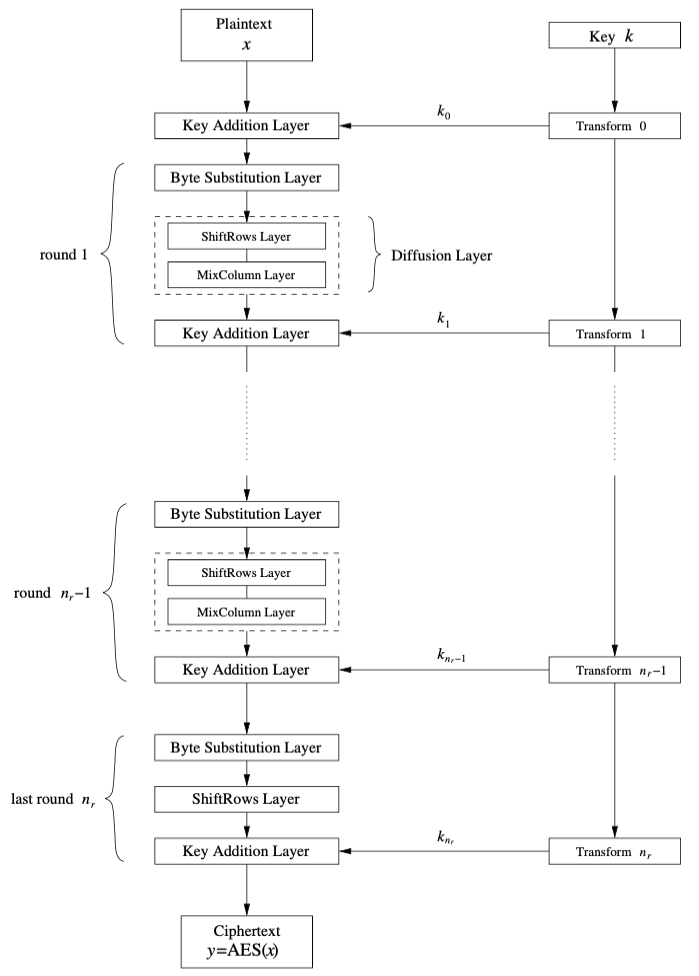
\includegraphics[width=.8\textwidth]{aes-block-diagram.png} % Adjust width as needed
    \caption{
        AES Encryption Block Diagram \cite{Paar2024}.
        The plaintext is denoted as $x$, the ciphertext as $y$, key as $k$, and the number of rounds as $n_r$.
    }
    \label{fig:aes-block-diagram}
\end{figure}